\documentclass[letterpaper, 10pt]{article}

\usepackage{amsmath}
\usepackage{float} 
\usepackage{graphicx}
\usepackage{gensymb}
\usepackage{array}


\usepackage[margin=1in]{geometry}

\title{Radio Background Research Notes}
\author{Nitika Yadlapalli}
\date{}


\begin{document}
\maketitle

\section{Sky Brightness Model for a Disk+Halo and Extragalactic Sources}

\subsection{Contribution from Disk}
Given a pair of galactic coordinates, we need to determine the line of sight through the disk. This, combined with the emission coefficient of the disk, will allow us to know the specific intensity contributed by the disk.

\begin{figure}[h]
\begin{center}
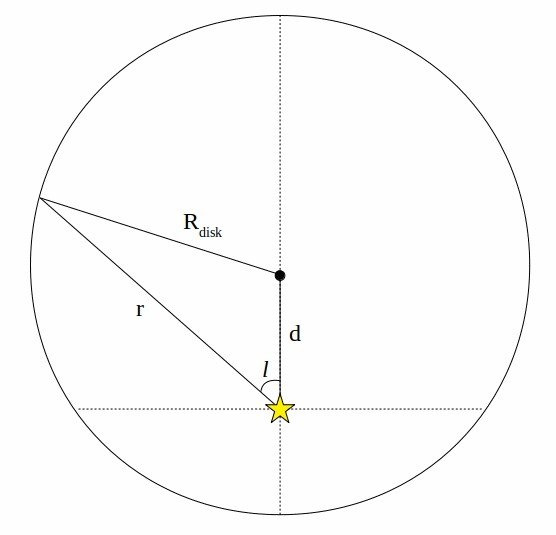
\includegraphics[width=0.39\textwidth]{disk_face.jpg}
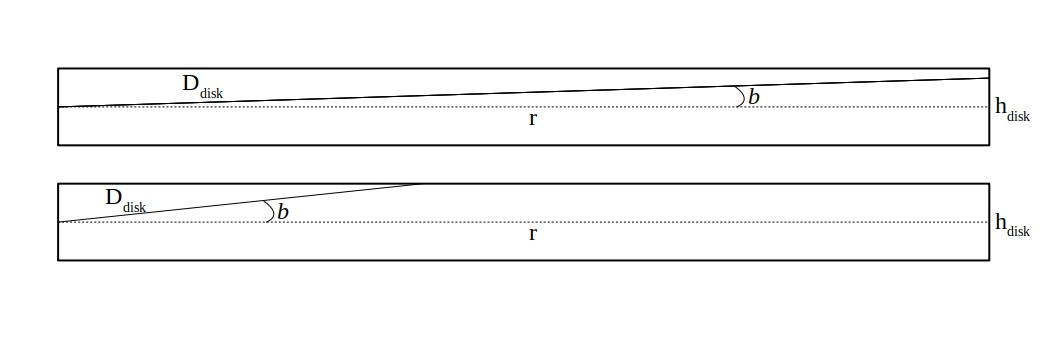
\includegraphics[width=0.59\textwidth]{disk_edge.jpg}
\caption{Two views of disk, face on and edge on, illustrating how line of sight through disk is calculated}
\label{disk}
\end{center}
\end{figure}

\begin{table}[h]
\centering
\begin{tabular}{| c | c |}
\hline
\textbf{Variable} & \textbf{Physical Meaning} \\
\hline
$D_{disk}$ & Total line of sight distance through disk \\
\hline
$R_{disk}$ & Radius of disk \\
\hline
$h_{disk}$ & Height of disk \\
\hline
$d$ & Distance between sun and galactic center \\
\hline
$l$ & Galactic longitude \\
\hline
$b$ & Galactic latitude \\
\hline
$r$ & Intermediate variable \\
\hline
\end{tabular}
\caption{Description of variables shown in Fig~\ref{disk}}
\end{table}

Referring to the left side of Fig~\ref{disk}, the yellow star represents the location of the solar system. The equations presented below will be for $ 0\degree < l < 180\degree $, as the results are symmetric for $ 180\degree < l < 360\degree $. First, making use of law of sines and law of cosines, I find that 

\[ r = \sqrt{R_{disk}^{2} + d^{2} - 2dR_{disk}cos\left[180 - l - sin^{-1}\left(\frac{dsin(l)}{R_{disk}}\right)\right]} \]

Then, given $r$, $D_{disk}$ can be given by one of two equations, depending on the value of $b$. 

\begin{table}[h]\
\centering
\begin{tabular}{c c}
$ D_{disk} = \frac{r}{cos(b)} $ & if $|b| < tan^{-1} \left(\frac{h/2}{r} \right)$ \\

$ D_{disk} = \frac{h}{sin(b)} $ & if $|b| > tan^{-1} \left(\frac{h/2}{r} \right)$ \\

\end{tabular}
\end{table}

Then, given an emission coefficient for the disk, 
\[I_{\nu, disk} = j_{\nu, disk}D_{disk} \]

In order to check these derived equations, we use example values approximated from the Subrahmanyan and Cowsik paper. A separate analysis will be done later to determine the model parameters that best fit our model to data. The disk model can be verified by plotting $ T_{b}\ vs\ csc(b)$, as shown in Figure~\ref{cscb} below. The plot is linear as expected for a correct model. A map of the brightness contributed just from the disk is shown in Figure~\ref{disk_map}.

\begin{figure}[h]
\begin{center}
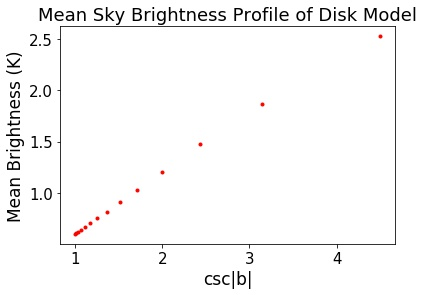
\includegraphics[width=0.5\textwidth]{cscb.jpg}
\caption{Plot of $ T_{b}\ vs\ csc(b)$}
\label{cscb}
\end{center}
\end{figure}

\begin{figure}[h]
\begin{center}
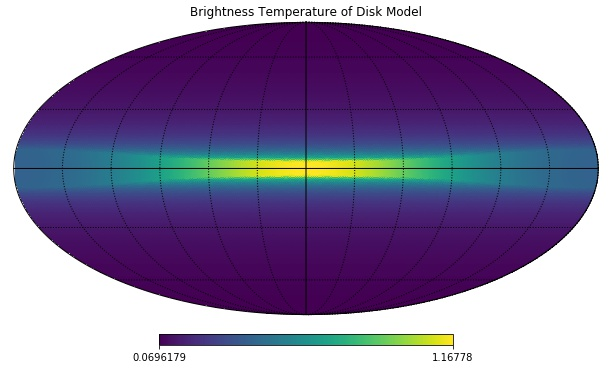
\includegraphics[width=0.6\textwidth]{disk.jpg}
\caption{Map of brightness temperature contributed by the disk}
\label{disk_map}
\end{center}
\end{figure}

\subsection{Contribution from Halo}
Next, we need to calculate the line of sight through the halo. Again, we only concern ourselves with angles in the range $ 0\degree < l < 180\degree $, as it will be symmetric in the range $ 180\degree < l < 360\degree $. To do that, we start by looking at the halo from the face on perspective, relative to the disk. Referring to the left side of Figure~\ref{halo}, we get both $d_{proj}$ and $R_{eff}$, which we need to solve for the entire line of sight through the disk.

\[ d_{proj} = d|cos(l)| \]

For $ l < 90\degree $, 
\[ R_{eff} + d_{proj} = \sqrt{R_{halo}^{2} + d^{2} - 2dR_{halo}cos\left[180 - l - sin^{-1}\left(\frac{dsin(l)}{R_{halo}}\right)\right]} \]

For $ l > 90\degree $, 
\[R_{eff} - d_{proj} = \sqrt{R_{halo}^{2} + d^{2} - 2dR_{halo}cos\left[180 - l - sin^{-1}\left(\frac{dsin(l)}{R_{halo}}\right)\right]} \]


\begin{figure}[h]
\begin{center}
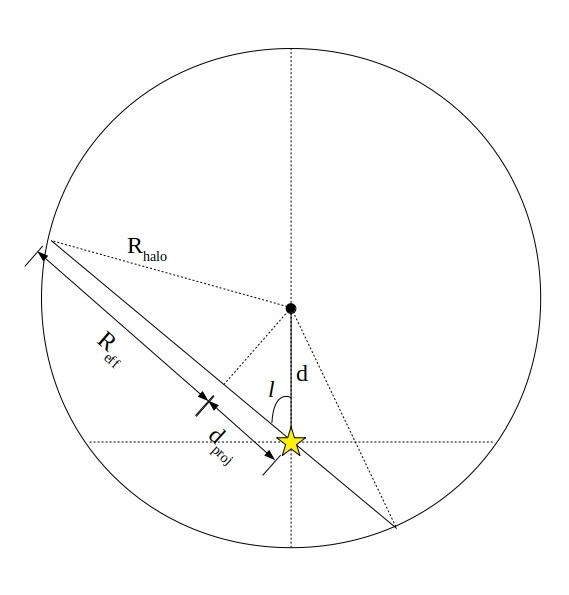
\includegraphics[width=0.495\textwidth]{halo_face.jpg}
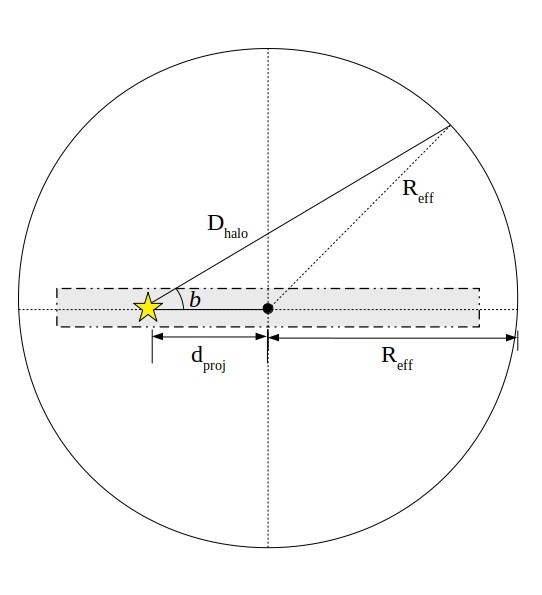
\includegraphics[width=0.485\textwidth]{halo_edge.jpg}
\caption{Two views of halo, face on and edge on (relative to the orientation of the disk), illustrating how line of sight through the halo is calculated. Shown above is an example for $ l < 90\degree$}
\label{halo}
\end{center}
\end{figure}

Next, we look at the halo edge on, relative to the disk, as shown in the right hand side of Figure~\ref{halo}.  For this example, if $ l < 90\degree$, 

\[ D_{halo} = \sqrt{R_{halo}^{2} + d_{proj}^{2} - 2R_{halo}d_{proj}cos\left[180 - b - sin^{-1}\left(\frac{d_{proj}sin(b)}{R_{halo}}\right)\right] }  \]

If $l > 90\degree$, 

\[ D_{halo} = \sqrt{R_{halo}^{2} + d_{proj}^{2} - 2R_{halo}d_{proj}cos\left[b - sin^{-1}\left(\frac{d_{proj}sin(b)}{R_{halo}}\right)\right] }  \]

Then, given an emission coefficient for the halo, 
\[I_{\nu, halo} = j_{\nu, halo}D_{halo} \]

A map of the brightness contributed just from the halo is shown in Figure~\ref{halo_map}, again using example values taken from the Subrahmanyan and Cowsik paper for the purpose of checking our derived equations.

\begin{figure}[h]
\begin{center}
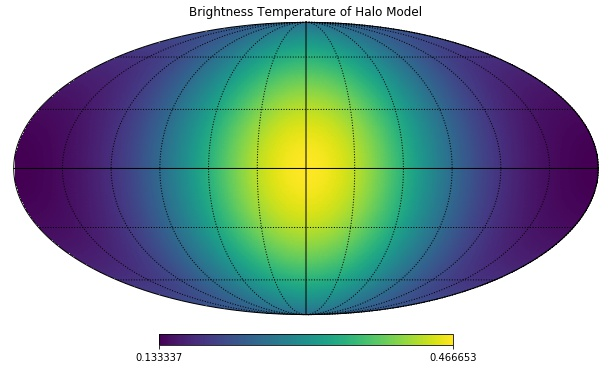
\includegraphics[width=0.6\textwidth]{halo.jpg}
\caption{Map of brightness temperature contributed by the halo}
\label{halo_map}
\end{center}
\end{figure}


\subsection{Extragalactic Source Counts}

Though plots showing source counts spanning over several orders of magnitude of brightness are shown in many papers, the analytic formulas and/or data points are scattered across the literature. In order to get the total sky brightness contributed by extragalactic sources, several models were combined. In the range of $0.05 - 1000\ mJy$ (equivalent to $10^{-5} - 1\ Jy$), can be modelled by the sixth order polynomial described by Hopkins et al (2002). The paper presents the result below, shown both analytically and graphically in Figure~\ref{Hopkins1}. In order to calculate the sky brightness, the curve shown in the right hand plot of Figure 6 must be integrated. 

\[ log\left(\frac{dN/dS}{S^{-2.5}}\right) = -0.008x^{6} + 0.057x^{5} - 0.121x^{4} - 0.049x^{3} + 0.376x^{2} + 0.508x + 0.859 \] \[x = log\left(\frac{S}{mJy}\right) \]

\begin{figure}[h]
\begin{center}
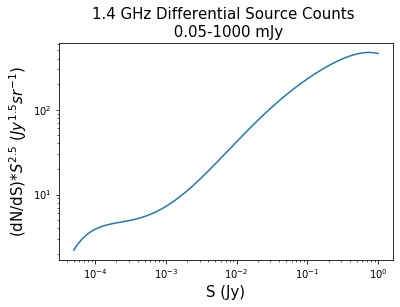
\includegraphics[width=0.49\textwidth]{Hopkins1.jpg}
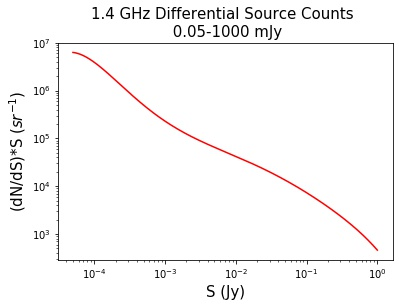
\includegraphics[width=0.49\textwidth]{Hopkins2.jpg}
\caption{Plot showing differential source counts at 1.4 GHz, as modelled in the Hopkins et al 2002 paper, described by $\frac{dN/dS}{S^{-2.5}}$ and a function of $S$ (left), and $S\left(dN/dS\right)$ as a function of $S$ (right), where $S$ is the sky brightness in $Jy$}
\label{Hopkins1}
\end{center}
\end{figure}

In the range of $0.011-44\ mJy$, Smolcic et al (2017), reports specific values for $\frac{dN/dS}{S^{-2.5}}$ at various sky brightnesses. Shown in Figure~\ref{Smolcic} is $S\left(dN/dS\right)$ as a function of $S$. The range of sky brightnesses for which source counts are reported somewhat overlap with the Hopkins paper. As expected, the graphs showing the source counts are consistent with each other.

\begin{figure}[h]
\begin{center}
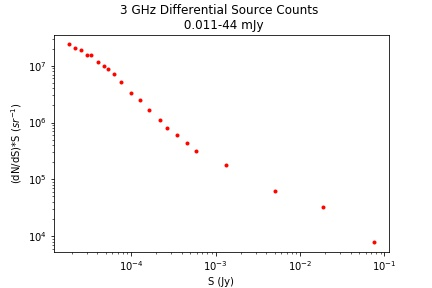
\includegraphics[width=0.49\textwidth]{Smolcic.jpg}
\caption{Plot showing differential source counts at 3 GHz, as modelled in the Smolcic et al (2017) paper, $S\left(dN/dS\right)$ as a function of $S$ }
\label{Smolcic}
\end{center}
\end{figure}

Finally, in the range of $ S < 10\ \mu Jy$, Condon et al 2012 predict that the source counts at 3.02 GHz are described as below. 

\[ \frac{dN}{dS} = 9000S^{-1.7}\ Jy^{-1}\ sr^{-1} \]


\begin{figure}[h]
\begin{center}
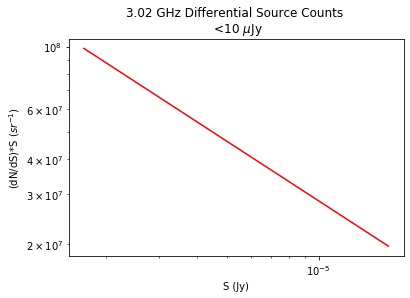
\includegraphics[width=0.49\textwidth]{Condon.jpg}
\caption{Plot showing differential source counts below $10\ \mu Jy$ at 3.02 GHz, as modelled in the Condon et al (2012) paper, $S\left(dN/dS\right)$ as a function of $S$ }
\label{Condon}
\end{center}
\end{figure}

As in this project, we'll be working with models of sky brightness at a particular frequency, we can use the following equation to transform $S$ into the frequency of our choice, where the spectral index is $ \alpha = -0.7$

\[ S_{f} = S_{i} \left(\frac{\nu_{f}}{\nu_{i}}\right)^{\alpha} \]

Total sky brightness is given by 
 \[ S_{tot} = \int \left(S\frac{dN}{dS}\right) dS \]
 
Total brightness temperature is given by the following equation. A plot representing the integrand is shown in Figure~\ref{Tb}.
 \[ T_{b} = \int \left(\frac{dT}{dS}\right) dS \ = \int \left(S\frac{dN}{dS}\right) \frac{c^{2}}{2\nu^{2}k} dS \]
 
\begin{figure}[h]
\begin{center}
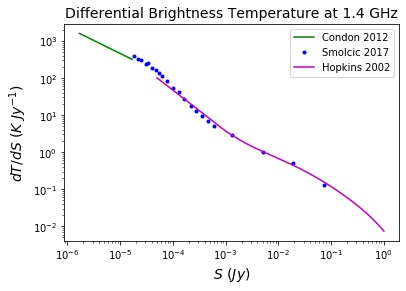
\includegraphics[width=0.59\textwidth]{T_b.jpg}
\caption{Differential brightness temperature plotted as a function of source brightness }
\label{Tb}
\end{center}
\end{figure}


 
\subsection{Masking Pixels in Central Latitudes}

Latitudes between $ -10\degree < b < 10\degree$ include emission from the galactic center that is not well understood. For our analysis, we wish to ignore these regions. Therefore, I have used \texttt{healpy}'s pixel querying function to set all of the pixels between these latitudes to \texttt{None}. The resulting map is shown in Figure~\ref{disk_mod}. Models masking only $ -5\degree < b < 5\degree$ were also run in order to better constrain parameters of the halo, but conclusive results have not been reached yet. 

\begin{figure}[h]
\begin{center}
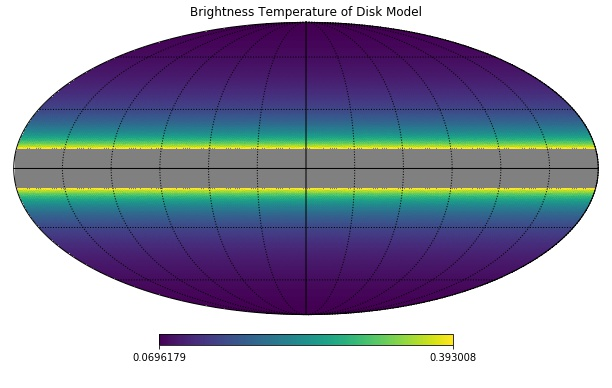
\includegraphics[width=0.6\textwidth]{disk_mod.jpg}
\caption{Map of brightness temperature contributed by the disk, with central latitudes ignored.}
\label{disk_mod}
\end{center}
\end{figure}


\section{Deriving Emission Coefficient from Brightness Temperature}
Given some brightness temperature, $T_{b}$, for both the halo and the disk (such as those given in the Subrahmanyan and Cowsik paper), I want to calculate the the emission coefficient (power per volume per steradian) for the disk and halo. To start, we can use the brightness temperature to calculate specific intensity using the Rayleigh Jeans approximation. 
\[ I_{\nu} = \frac{2\nu^{2}}{c^{2}}kT_{b} \]

From there, see Chapter 1 of \emph{Radiative Processes} by Rybicki and Lightman for the following equation relating specific intensity and emission coefficient. 

\[ dI_{\nu} = j_{\nu}ds  \]

Assuming that $j_{\nu}$ is constant along all lines of sight and given a line of sight distance $D$, 

\[ I_{\nu} = j_{\nu}D \]

Given this, the emission coefficient for the spherical galactic halo is given by 

\[j_{\nu, halo} = \left(\frac{2\nu^{2}}{c^{2}}kT_{b, halo}\right)\left(\frac{1}{R_{halo}}\right)\]

while the emission for a disk is given by 
\[j_{\nu, disk} = \left(\frac{2\nu^{2}}{c^{2}}kT_{b, disk}\right)\left(\frac{1}{R_{disk}}\right)\]

Then, the specific intensity along a line of sight can be given by 

\[I_{\nu} = j_{\nu, halo}D_{halo} + j_{\nu, disk}D_{disk} \]

\section{Fitting Model Parameters}
This section describes our methods for fitting model parameters to all sky maps downloaded from LAMBDA (https://lambda.gsfc.nasa.gov/). In order to calculate model paramters that best fit the data, we use Python package \texttt{emcee}. 

\subsection{Minimizing the Minimum of Residuals}
In our first attempt to fit our model to data, we assumed brightness contributions from a disk, extragalactic sources, and the CMB. Our likelihood function first calcualted residuals as a function of $l$ and $b$ as follows

\[ T_{residual}(l,b) = T_{sky}(l,b) - T_{disk}(l,b) - T_{extragalactic} - T_{CMB} \]

To calculate our likelihood, we then assumed

\[ S = min\left(|T_{residual}(l,b)|\right) \] 

and 

\[ L\ \propto\ exp\left[-\frac{S^2}{2T_{rms}^2}\right] \]

For this test, I downloaded the 1.4 GHz all sky map made by the Stockert and Villa-Elisa telescopes. The $3\sigma\ T_{rms}$ is reported to be 50 mK for this 1.4 GHz map. As the resolution of this map is quite high, \texttt{hp.pixelfunc.ud\_grade} is used downgrade the resolution, which speeds up the calculations. This model was not successful in predicting the model parameters, as creating a statistic based on only one pixel per sky map is unreliable. 

\subsection{Measuring Gaussianity of Residuals}
Using the value of a single pixel as a statistic, as described in section 3.1, was poorly constraining. Additionally, it prefers a model where the minimum pixel value is zero, which is problematic as that means more emission than just noise is being left in the residuals. For an ideal model, the sky temperature minus the model temperature should just leave Gaussian noise. In reality, it is impossible for our rudimentary models to subtract precise structure, so we will be left with more positive residuals than negative. The residuals should follow a right-tailed distribution, where the negative residuals resemble half a Gaussian and the positive residuals include residual emission caused by Galactic structure. Taking this into account, our new likelihood will be a statistic determining how likely it is that our negative residuals are Gaussian. In order to do this, we employ the Kolmogorov-Smirnov test (KS test). This test measures the maximum distance between the cummulative distribution function of the residuals and an empirical distribution function (EDF). The empirical distribution function is calculated as such: given an ordered dataset $\left[x_1, x_2, ..., x_n,...,x_{N-1}, x_N\right] $, the EDF at every point is given by

\[EDF = \frac{n}{N}\]

An example of this is given in Figure~\ref{edf} for a set of 5000 random numbers generated in a Gaussian distribution with a mean of 0 and a standard devitation of 1. 

\begin{figure}[h]
\begin{center}
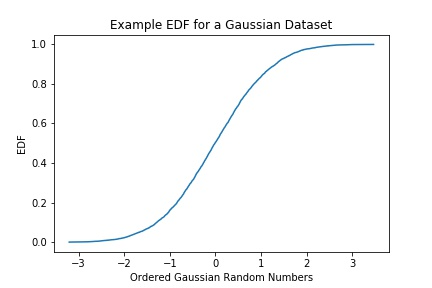
\includegraphics[width=0.6\textwidth]{EDFexample.jpg}
\caption{An empirical distribution function created for a set of Gaussian random numbers}
\label{edf}
\end{center}
\end{figure}

The test statistic, given by $\sqrt{N}D$, where $D$ is the maximum distance between the two functions given a dataset with $N$ samples, is then assigned a p-value that describes the likelihood of the data being Gaussian. The probability distribution function (PDF) as a function of the test statistic is shown in the left side of Figure~\ref{kspdf}. The p-value for each point is calculated by 

\[p = 1 - \int_{0}^{\sqrt{N}D} PDF(x)\ dx \]

A graph of the p-value as a function of statistic is shown in the right side of Figure~\ref{kspdf}. As the p-value increases with a decreasing test statistic, we felt it was a suitable quantity to represent how Gaussian our negative resdiuals were and we felt justified in using the p-value as our likelihood. 


\begin{figure}[H]
\begin{center}
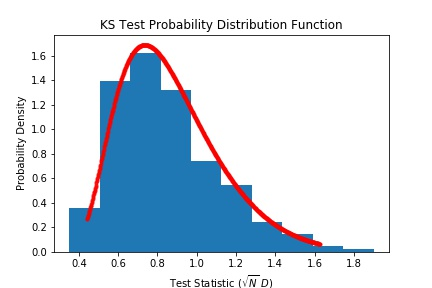
\includegraphics[width=0.49\textwidth]{kstestPDF.jpg}
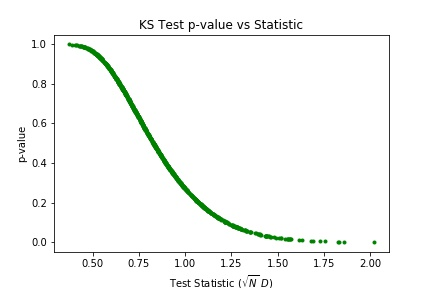
\includegraphics[width=0.49\textwidth]{kstest_pvaluedist.jpg}
\caption{KS test probability density and p-values as a function of the test statistic $\sqrt{N}D$}
\label{kspdf}
\end{center}
\end{figure}

\begin{figure}[h]
\begin{minipage}{.5\textwidth}
\centering
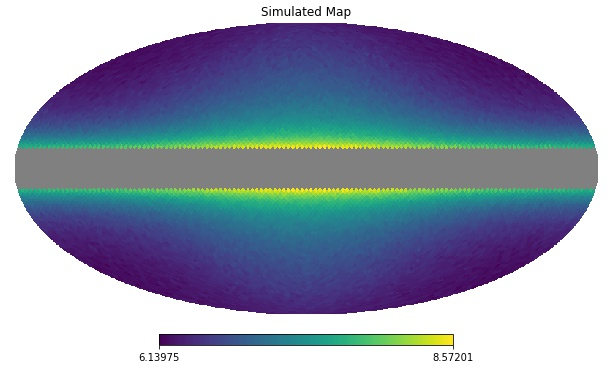
\includegraphics[height=0.75\textwidth]{simulated_map.jpg}
\end{minipage}%
\begin{minipage}{0.5\textwidth}
\centering

\hfill


\renewcommand{\arraystretch}{1.5}
\begin{tabular}{|>{\centering\arraybackslash}m{1.75cm}|>{\centering\arraybackslash}m{1.75cm}|}
\hline
Quantity & Value \\
\hline
$R_{disk}$ & $1.5d$ \\
\hline
$h_{disk}$ & $0.2d$ \\
\hline
$j_{disk}$ & $10^{-40}$ \\
\hline
$R_{halo}$ & $3.0d$ \\
\hline
$j_{halo}$ & $10^{-41}$ \\
\hline
$T_{bkg}$ & $2.0$ \\
\hline

\end{tabular}
\renewcommand{\arraystretch}{1}
\end{minipage}

\caption{Simulated sky map and parameters that went into the simulation. Some random noise was also added to this map.}
\end{figure}


To prove the viability of this method, I first tested it out on a simulated sky map. The sky map, shown in the left side of Figure~13, was created with a disk, halo, uniform background, CMB, and extragalactic component. Given the solar circle, $d$, the values fed into the simulated map are shown in the table in Figure~13. 

\newpage

\begin{figure}[H]
\begin{center}
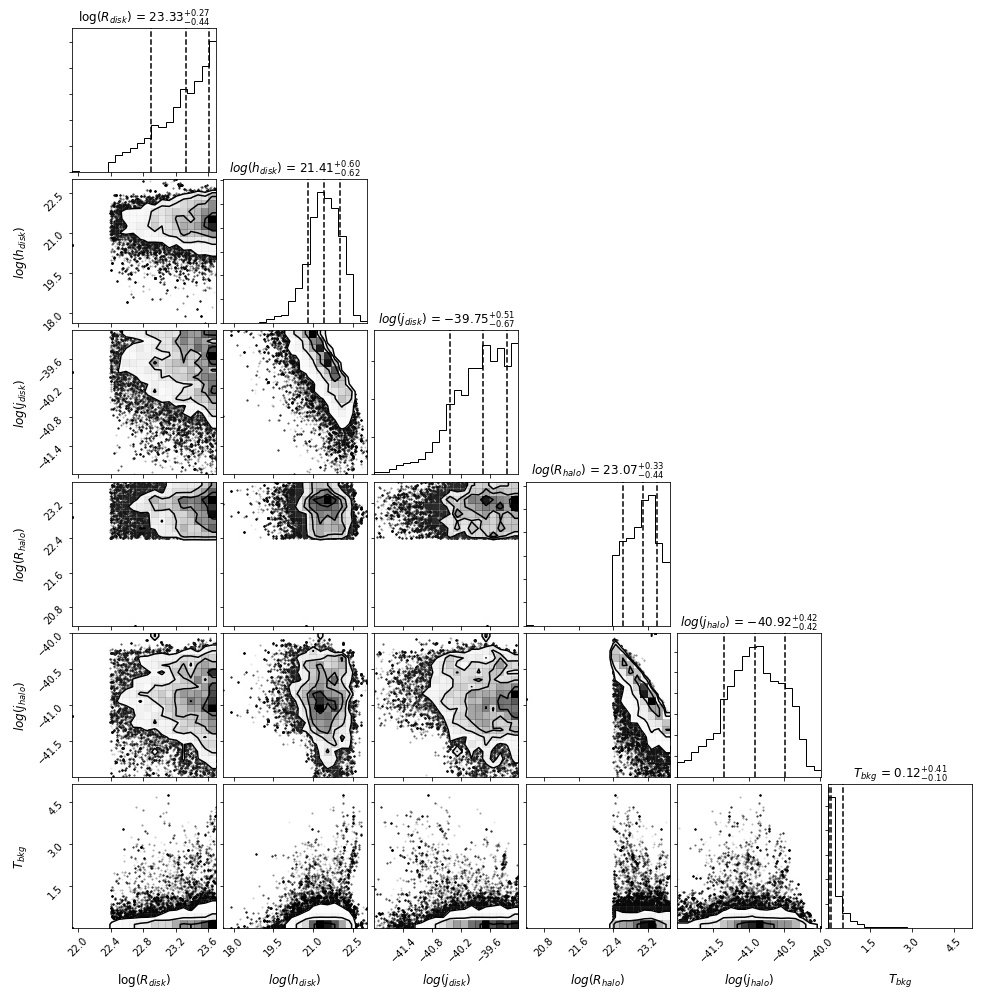
\includegraphics[width=\textwidth]{corner_simdata.jpg}
\caption{Corner plot showing the results from the MCMC analysis of the simulated map.}
\label{mcmcsim}
\end{center}
\end{figure}

The results of the MCMC run to extract the parameters from the simulated map are shown in Figure~\ref{mcmcsim}. The plot shows that our analysis failed to constrain values for the radius of the disk as well as the temperature of the background. The emission coefficient of the disk is also poorly constrained. The remaining values have been correctly extracted within the error bars, though our model prefers increased emission from the disk and halo and no background temperature. The model also correctly plotted an anticorrelation between $h_{disk}$ and $j_{disk}$ as well as $R_{halo}$ and $j_{halo}$. Though not perfect, we decided to try and run the same analysis on the real sky map. I ran three models: disk+background, disk+halo, and disk+halo+background.

\newpage

\begin{figure}[H]
\begin{center}
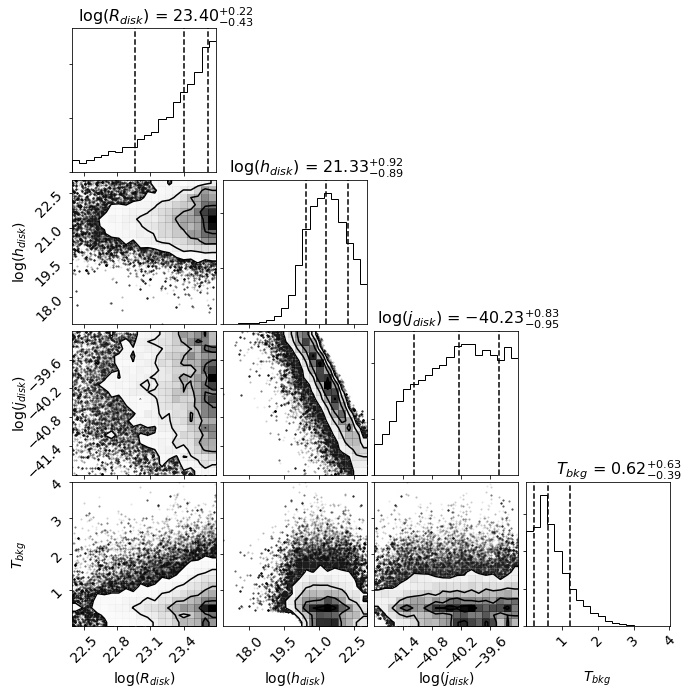
\includegraphics[width=\textwidth]{corner_disk+bkg.jpg}
\caption{Corner plot showing the results from the MCMC analysis assuming a disk and uniform background model for the galaxy.}
\label{corner_disk+bkg}
\end{center}
\end{figure}

Figure~\ref{corner_disk+bkg} shows the corner plot for the model of the sky with a disk and uniform background. This plot again shows that the radius of the disk is poorly constrained. The main reason for this is because the all sky maps we fit to have the middle 20$\degree$ blocked out, so the areas of the disk that are affected by an increase in radius make no appearance in the residuals. Encouragingly, the anticorrelation between the disk height and emission coefficient is recovered. The background temperature has the highest probability to be around 0.65 K. Because of this, we can say that a model including a halo should be run to confirm or deny whether or not a halo is causing this excess temperature.

\newpage

\begin{figure}[H]
\begin{center}
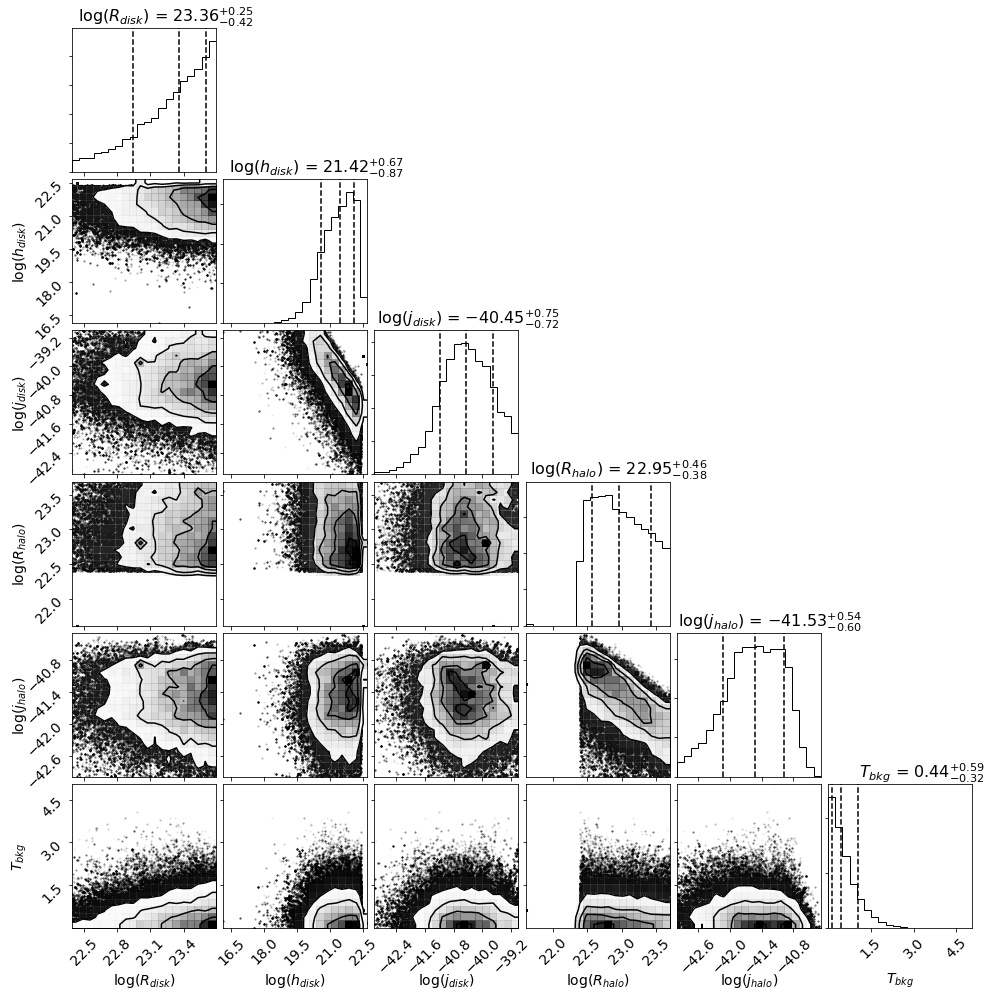
\includegraphics[width=\textwidth]{corner_disk+halo+bkg.jpg}
\caption{Corner plot showing the results from the MCMC analysis assuming a disk, halo, and uniform background model for the galaxy.}
\label{corner_disk+halo+bkg}
\end{center}
\end{figure}

\newpage

\begin{figure}[H]
\begin{center}
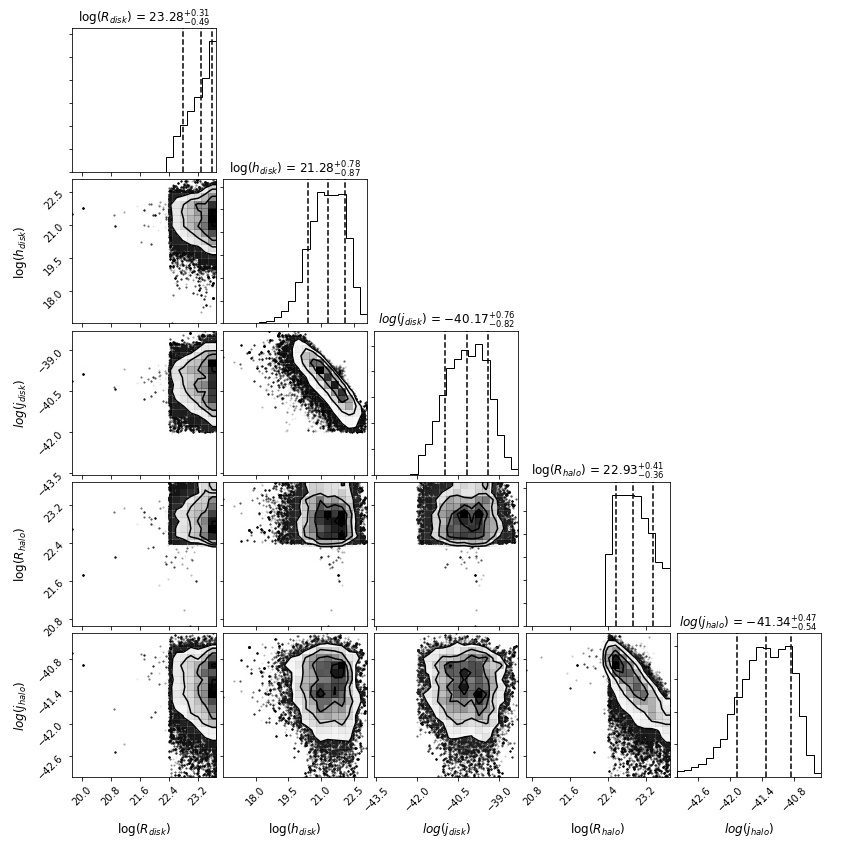
\includegraphics[width=0.93\textwidth]{corner_disk+halo.jpg}
\caption{Corner plot showing the results from the MCMC analysis assuming only a disk and halo model for the galaxy (no uniform background).}
\label{corner_disk+halo}
\end{center}
\end{figure}

Looking at Figure~\ref{corner_disk+halo+bkg}, the background temperature looks to have been selected to be 0 most often. This raises the question of whether an extra background temperature exists with the halo included in the model. That is, does the halo explain the excess seen in the disk+background only model? To test this, I ran another model without the uniform background as a free parameter. The results of that analysis are shown in Figure~\ref{corner_disk+halo}. All of the inferred values for this model are consistent with the disk+halo+background model within 1$\sigma$, which could indicate that the halo accounts for any excess temperature present in models without the halo. Doing a test for model selection, such as calculating the BIC, for each of these models could provide more insight on whether or not a background temperature makes a significant difference in the residuals. 

Still, this does not provide any conclusive evidence for the presence of the halo. It only says for certain that a disk model is not enough to explain all of the observed emission at these frequencies. A difficulty in this approach is that there is a lot of galactic foreground left in the residuals and it is hard to properly model the structure of the foreground to include in our analysis. Thus, we decided to use a different approach to subtract the galactic foreground, explained in the following section.

\subsection{Subtracting Galactic Foreground via Methods Outlined by TRIS Team}
TRIS, similar to ARCADE, is a low frequency balloon experiment that aimed to measure fluctutations in the CMB that would be harder to detect at higher frequencies used by experiments such as COBE, WMAP, and \emph{Planck}. TRIS utilized three absolutely calibrated radiometers at the following frequencies: 0.60 GHz, 0.82 GHz, and 2.5 GHz. However, strong and persistent RFI in the 2.5 GHz radiometer makes the observations unusable. 

$\alpha_{1}$





\end{document}
